\documentclass{article}

% - style template
\usepackage{base}

% - title, author, etc.
\title{COMP3007 - Assignment}
\author{Tom Ross}
\date{\today}

% - headers
\pagestyle{fancy}
\fancyhf{}
\rhead{\theauthor}
\chead{}
\lhead{\thetitle}
\rfoot{\thepage}
\cfoot{}
\lfoot{}

% - document
\begin{document}

The entire code repository can be found at
\url{https://github.com/dgsaf/comp3007_assignment}.

\tableofcontents

\listoffigures

\listoftables

\clearpage

\section{Introduction}
\label{sec:introduction}

\section{Problem Analysis}
\label{sec:problem-analysis}

We are concerned with the detection and classification of two similar but
distinct types of signs.
The properties specific to each type of signage are discussed in
\autoref{sec:problem-1} and \autoref{sec:problem-2}.
Here, we remark on the properties common to both of them, which are numerous and
allow for a broadly unified approach to their detection and classification.

Each sign consists of a black background with white characters (digits and
directional arrows) forming the foreground of the sign.
The black background is rectangular in shape, and bounds the characters
regions.
Furthermore, the contrast between the black background and the white foreground
is strong across all colour channels and in grayscale.

The digits are uniform in their construction, being printed in a monospace
font with fixed height and allocated a fixed width; although each digit does
not necessarily fully extend across its allocated width - as can be seen for the
digit 1.
Likewise, the directional arrows are also uniform in their construction but
their dimensions are distinct from those of the digits - noticeably having a
smaller height than the digits.

The digits do not overlap with each other (unless subject to camera
artifacts/blurring) but are closely adjacent to each other, and regularly
spaced.
Each sign contains at least one sequence of three digits, which are ideally
surrounded by a black sub-region of the sign; although for task 2, the gap
between the leftmost digit and the edge of the sign can be very small.

In summary, the following properties of the signs are almost always observed,
providing a robust foundation for their detection:
\begin{itemize}
\item
  The uniformly white colour of the characters;

\item
  The uniformly black background of the sign;

\item
  The strong contrast between the white characters and the black background
  across all red, green, and blue channels as well as in grayscale;

\item
  The uniform height of the digits;

\item
  The uniform spacing of the characters horizontally;

\item
  The height of the digits exceeding the width;

\item
  The uniform dimensions of the arrows;

\item
  The presence of a chain of exactly three digits;

\item
  A sizeable sub-region of the sign above and below the chain of digits, which
  is uniformly black.
\end{itemize}
However, the assumption of the above properties may be invalidated by any one of
the (non-exhaustive) list of conditions:
\begin{itemize}
\item
  The presence of strong radial, or motion blurring which may cause character to
  overlap;

\item
  The presence of strong shadowns, glare, or other variations in lighting
  conditions across the character;

\item
  The presence of a foreign object, such as a sticker or a mark, on the sign
  (violating the assumptions on uniformity of layout) or across the characters
  (violating the assumptions on uniformity of characters).

\end{itemize}
It should also be noted that often there are other monospace white characters
present near the sign - typically letters forming the name of the location
marked by the sign.
These characters can be distinguished from the digits (and arrows) by the fact
that they almost always form chains of more than three characters, and presented
on their own signs which almost never have a black background.

\subsection{Task 1}
\label{sec:problem-1}

Further refinement of the problem analysis is possible for task 1.
We are concerned with finding only one chain of three digits, and we are not
concerned with directional arrows at all.
Futhermore, there exists a sizeable gap between the chain of digits and the edge
of the sign both horizontally and vertically.

Bricks and other objects which are of approximately uniform dimensions and
uniformly spaced are regularly present in images for task 1 - hence, when
exploiting the uniformity of the layout of the digits, care must be taken to
avoid or handle the false detection of these other objects.

Examples of the images expected for task 1, which provide the justification for
the assumptions made on the properties of the sign are shown in
\autoref{fig:problem-1-regular}.
Examples of images which may be encountered for task 1, but which challenge the
assumptions made on the properties of the sign are shown in
\autoref{fig:problem-1-outlier}.

\begin{figure}[h]
  \centering
  \begin{subfigure}[h]{0.22\textwidth}
    \centering
    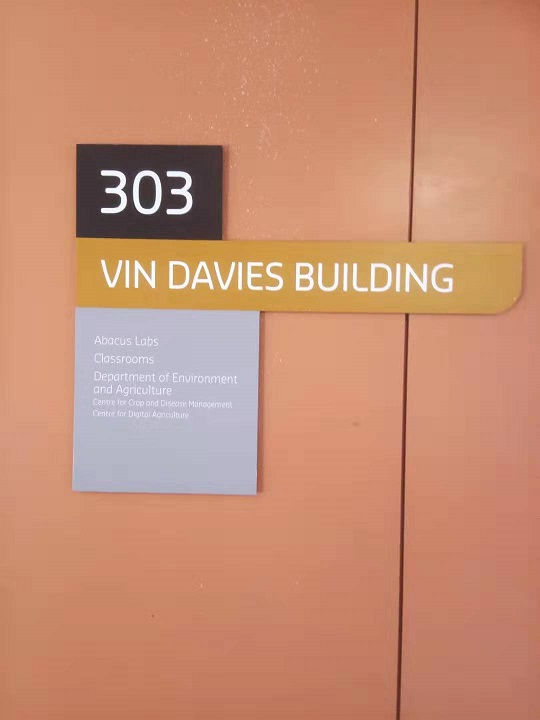
\includegraphics[width=0.9\textwidth]{../train/task1/BS02}
    \caption[BS02]{
      \lstinline{BS02.jpg}
    }
    \label{fig:bs02}
  \end{subfigure}
  %
  \begin{subfigure}[h]{0.22\textwidth}
    \centering
    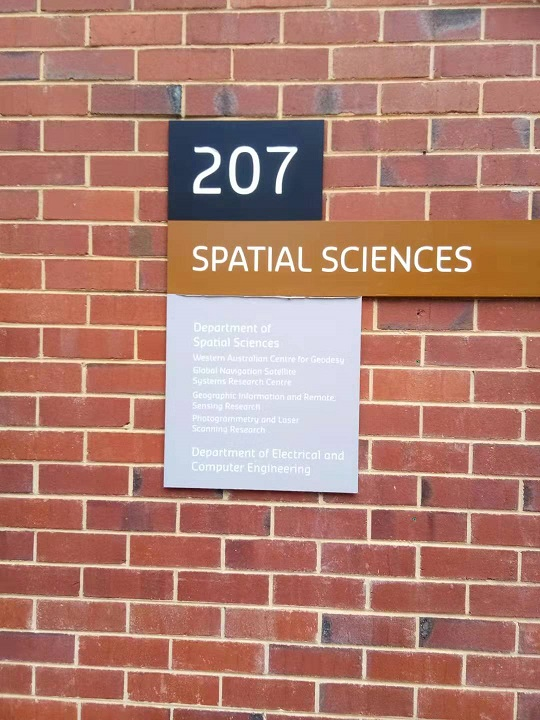
\includegraphics[width=0.9\textwidth]{../train/task1/BS04}
    \caption[BS04]{
      \lstinline{BS04.jpg}
    }
    \label{fig:bs04}
  \end{subfigure}
  %
  \begin{subfigure}[h]{0.22\textwidth}
    \centering
    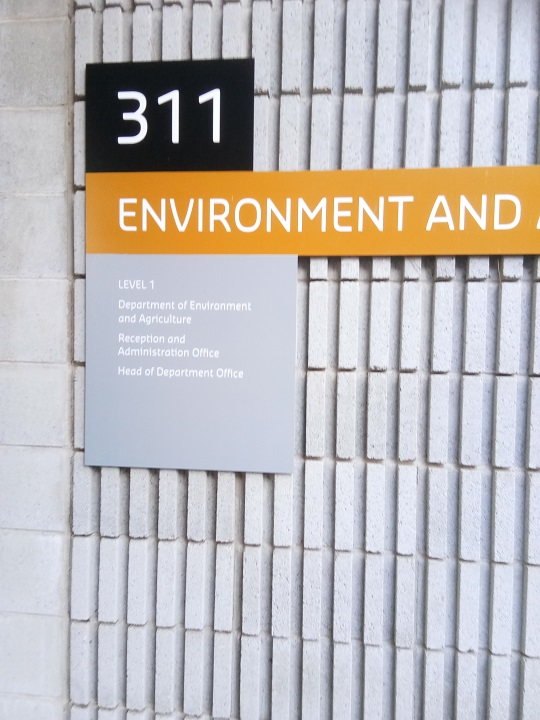
\includegraphics[width=0.9\textwidth]{../train/task1/BS09}
    \caption[BS09]{
      \lstinline{BS09.jpg}
    }
    \label{fig:bs09}
  \end{subfigure}
  %
  \begin{subfigure}[h]{0.22\textwidth}
    \centering
    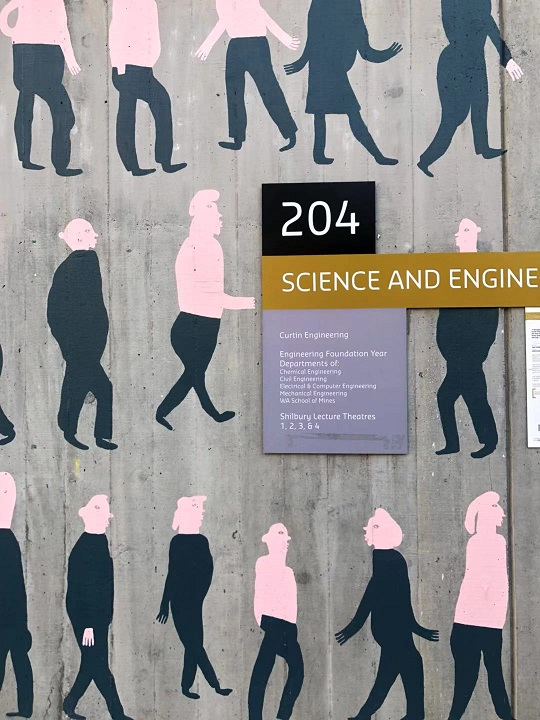
\includegraphics[width=0.9\textwidth]{../train/task1/BS14}
    \caption[BS14]{
      \lstinline{BS14.jpg}
    }
    \label{fig:bs14}
  \end{subfigure}

  \caption[Task 1 - Regular Cases]{
    Examples of training images for task 1, which exhibit the described
    distinguishing properties of the signs and digits.
  }
  \label{fig:problem-1-regular}
\end{figure}

\begin{figure}[h]
  \centering
  \begin{subfigure}[h]{0.22\textwidth}
    \centering
    
\includegraphics[width=0.9\textwidth]{../train/task1/BS03}
    \caption[BS03]{
      \lstinline{BS03.jpg}
    }
    \label{fig:bs03}
  \end{subfigure}
  %
  \begin{subfigure}[h]{0.22\textwidth}
    \centering
    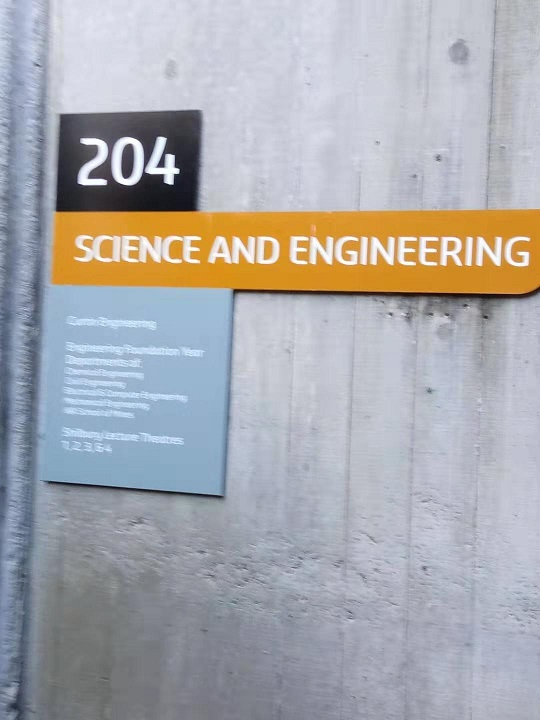
\includegraphics[width=0.9\textwidth]{../train/task1/BS05}
    \caption[BS05]{
      \lstinline{BS05.jpg}
    }
    \label{fig:bs05}
  \end{subfigure}
  %
  \begin{subfigure}[h]{0.22\textwidth}
    \centering
    
\includegraphics[width=0.9\textwidth]{../train/task1/BS07}
    \caption[BS07]{
      \lstinline{BS07.jpg}
    }
    \label{fig:bs07}
  \end{subfigure}
  %
  \begin{subfigure}[h]{0.22\textwidth}
    \centering
    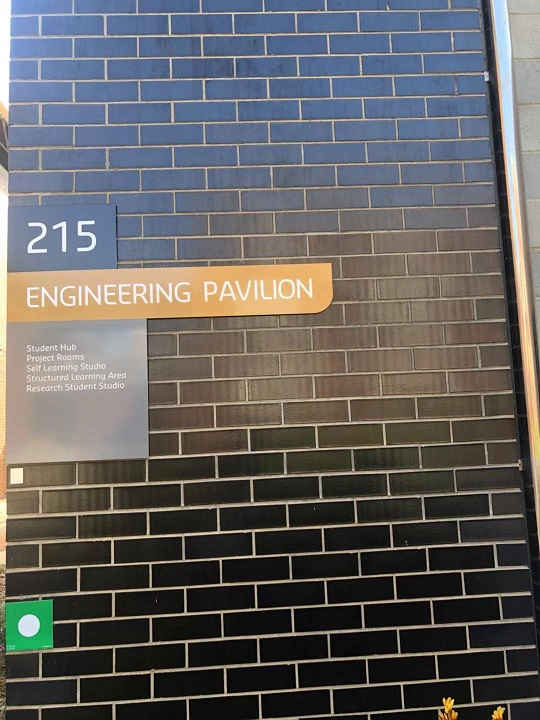
\includegraphics[width=0.9\textwidth]{../train/task1/BS11}
    \caption[BS11]{
      \lstinline{BS11.jpg}
    }
    \label{fig:bs11}
  \end{subfigure}

  \caption[Task 1 - Edge Cases]{
    Examples of training images for task 1, which may challenge the assumptions
    made on the signs and thus necessitate the development of a robust detection
    algorithm.
    Sharp shadows, motion blur and monochromatic periodic objects, which may
    interfere with digit detection, can be observed.
  }
  \label{fig:problem-1-outlier}
\end{figure}

\subsection{Task 2}
\label{sec:problem-2}

Similarly, further refinement of the problem analysis is possible for task 2.
We are concerned with finding a variable number of chains of three digits, each
of which has an associated directional arrow to their right.
For each chain and their associated directional arrow, the geometric centres of
the digits are arrow are collinear; hence we say that they form a line.
Each line is vertically spaced (by a distance just larger than the height of the
digits) and the set of digits and arrows from each line thus forms a grid-like
layout.

A challenging aspect of these signs, compared to those for task 1, is that the
gap between the leftmost digit on each line and the edge of the sign can be very
small.
In cases where an object, of similar colour/intensity to the white characters,
is behind the sign but in a similar region of the image to the leftmost digit of
a line, the digit and the object may prove difficult to distinguish as separate
regions.

Another difficulty is that the number of lines in any particular sign is not
known beforehand.
However, there is a benefit in having multiple lines per sign as it provides a
mechanism, given at least one fully known line or even partial information from
multiple lines, to recover an expected location for characters which fail to be
detected initially.

Similar to task 1, the scene environment can be expected to be quite noisy, with
periodically repeating objects such as brickwork present, as well as other
objects with many sharp edges, such as plants and trees.
It also seen that foreign objects, such as stickers and marks, may be present on
the signs, and that other objects, such as plants, may occlude the sign itself.

Examples of the images expected for task 2, which provide the justification for
the assumptions made on the properties of the sign are shown in
\autoref{fig:problem-2-regular}.
Examples of images which may be encountered for task 2, but which challenge the
assumptions made on the properties of the sign are shown in
\autoref{fig:problem-2-outlier}.

\begin{figure}[h]
  \centering
  \begin{subfigure}[h]{0.22\textwidth}
    \centering
    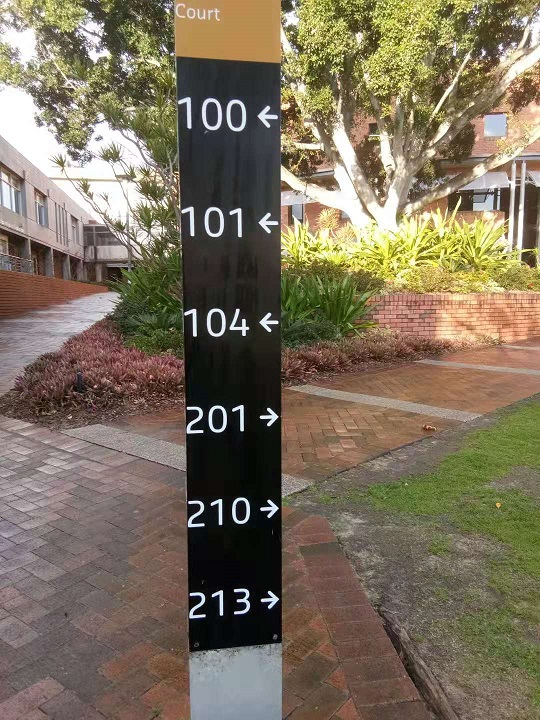
\includegraphics[width=0.9\textwidth]{../train/task2/DS06}
    \caption[DS06]{
      \lstinline{DS06.jpg}
    }
    \label{fig:ds06}
  \end{subfigure}
  %
  \begin{subfigure}[h]{0.22\textwidth}
    \centering
    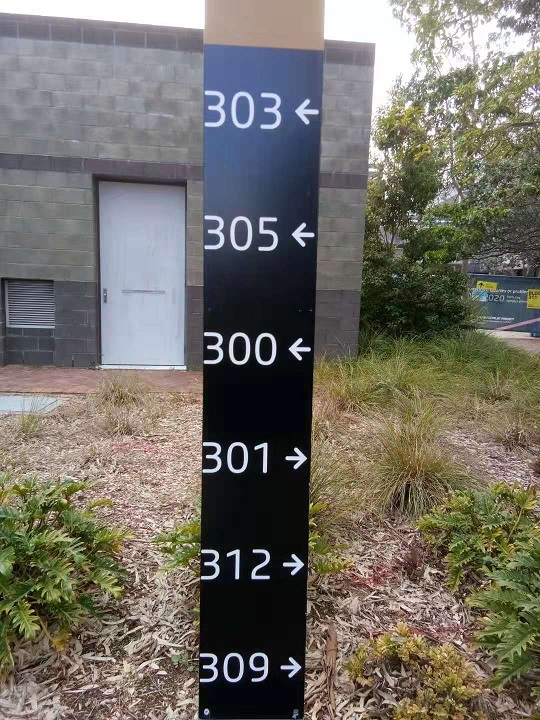
\includegraphics[width=0.9\textwidth]{../train/task2/DS12}
    \caption[DS12]{
      \lstinline{DS12.jpg}
    }
    \label{fig:ds12}
  \end{subfigure}
  %
  \begin{subfigure}[h]{0.22\textwidth}
    \centering
    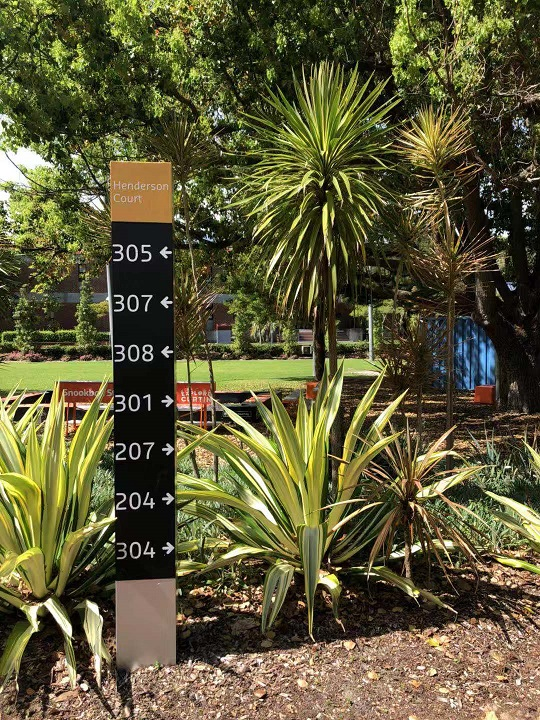
\includegraphics[width=0.9\textwidth]{../train/task2/DS13}
    \caption[DS13]{
      \lstinline{DS13.jpg}
    }
    \label{fig:ds13}
  \end{subfigure}
  %
  \begin{subfigure}[h]{0.22\textwidth}
    \centering
    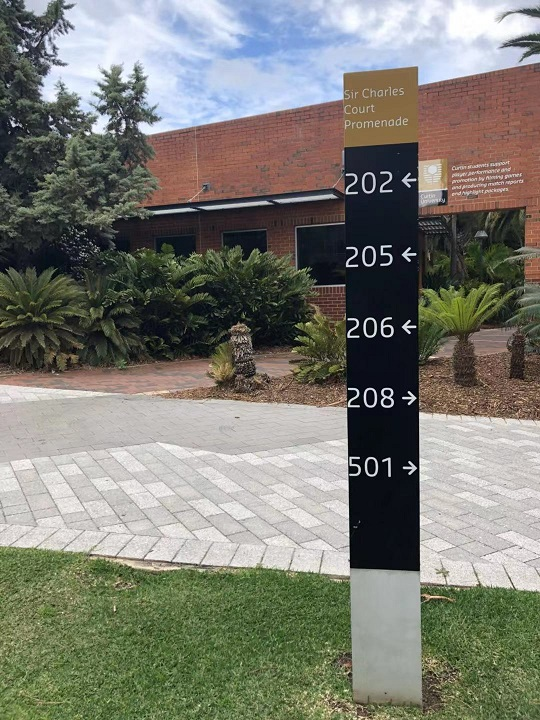
\includegraphics[width=0.9\textwidth]{../train/task2/DS18}
    \caption[DS18]{
      \lstinline{DS18.jpg}
    }
    \label{fig:ds18}
  \end{subfigure}

  \caption[Task 2 - Regular Cases]{
    Examples of training images for task 2, which exhibit the described
    distinguishing properties of the signs, and their digits and arrows.
  }
  \label{fig:problem-2-regular}
\end{figure}

\begin{figure}[h]
  \centering
  \begin{subfigure}[h]{0.22\textwidth}
    \centering
    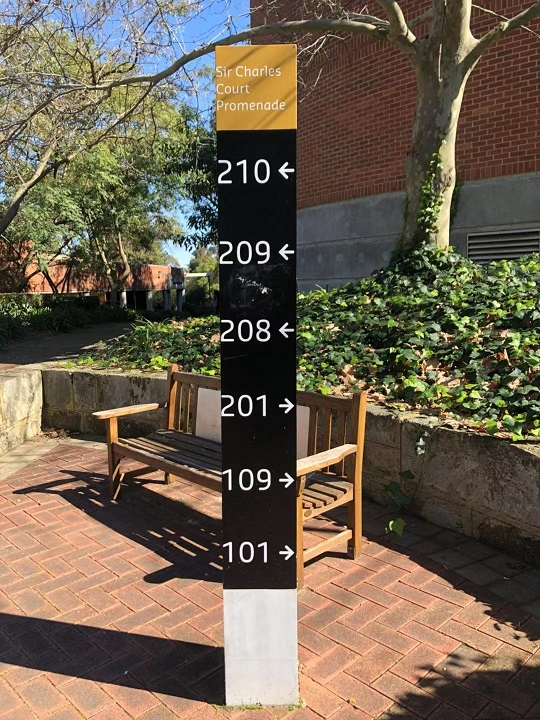
\includegraphics[width=0.9\textwidth]{../train/task2/DS02}
    \caption[DS02]{
      \lstinline{DS02.jpg}
    }
    \label{fig:ds02}
  \end{subfigure}
  %
  \begin{subfigure}[h]{0.22\textwidth}
    \centering
    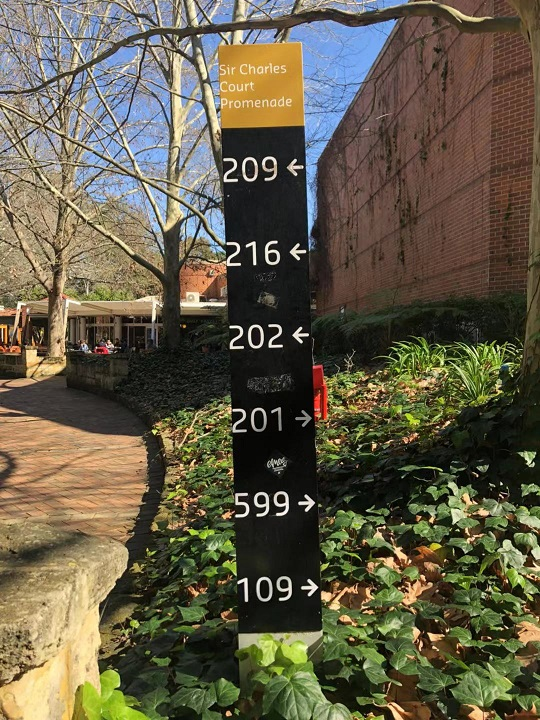
\includegraphics[width=0.9\textwidth]{../train/task2/DS07}
    \caption[DS07]{
      \lstinline{DS07.jpg}
    }
    \label{fig:ds07}
  \end{subfigure}
  %
  \begin{subfigure}[h]{0.22\textwidth}
    \centering
    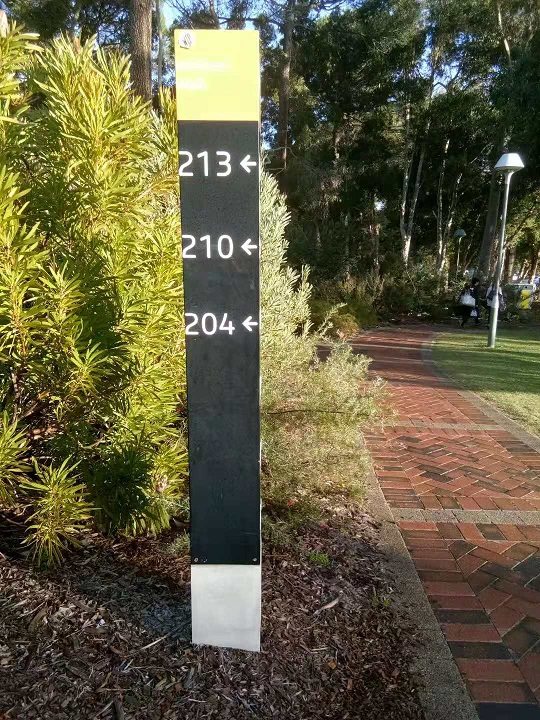
\includegraphics[width=0.9\textwidth]{../train/task2/DS10}
    \caption[DS10]{
      \lstinline{DS10.jpg}
    }
    \label{fig:ds10}
  \end{subfigure}
  %
  \begin{subfigure}[h]{0.22\textwidth}
    \centering
    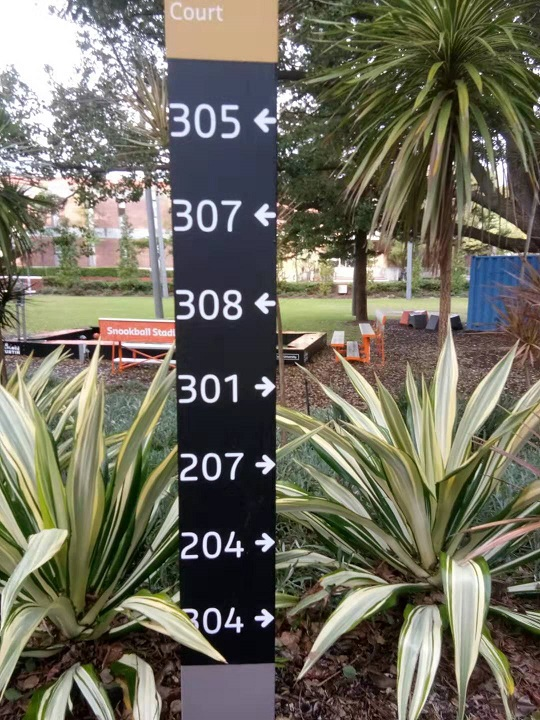
\includegraphics[width=0.9\textwidth]{../train/task2/DS11}
    \caption[DS11]{
      \lstinline{DS11.jpg}
    }
    \label{fig:ds11}
  \end{subfigure}

  \caption[Task 2 - Edge Cases]{
    Examples of training images for task 2, which may challenge the assumptions
    made on the signs and thus necessitate the development of a robust detection
    algorithm.
    Characters overlapping with similar regions outside the sign, foreign
    objects on the sign, variable lighting conditions can all be observed.
  }
  \label{fig:problem-2-outlier}
\end{figure}

\clearpage

\section{Implementation}
\label{sec:imp}

\subsection{Overview}
\label{sec:imp-overview}

We make use of the commonality of the properties of the signs that are to be
detected in task 1 and task 2 by designing a detection algorithm which can be
adapted with minor changes for each task.
The specific detection algorithms for each task are discussed in
\autoref{sec:imp-1} and \autoref{sec:imp-2}.
Furthermore, as the digits to be classified in each task are of the same style,
we also design a classification algorithm which is suitable for both tasks.
Naturally, a separate classifier will be needed for the directional arrows,
however we use the $k$-Nearest Neighbours ($k$-NN) algorithm for classifying
both the digits and the arrows.
Hence, we discuss the problem of classification, for both types of characters,
in a general manner in \autoref{sec:imp-classification}.

To detect the characters (digits and arrows) we utilise the method of
Maximally Stable Extremal Regions (MSER) - first developed by
\cite{MATAS2004761}.
We present our formalism in a similar manner to \cite{MATAS2004761}.
In this method, a number of regions, which are extremal in terms of light
intensity and stable in the sense that the region boundary changes little under
a varying threshold, are detected in the grayscale image.
With suitably chosen parameters for the MSER algorithm, the regions of interest,
corresponding to the characters on the sign, can be reliably detected - but must
be distinguished from the other regions detected which are not of interest.
Using known properties of the characters (such as dimension, aspect ratio,
bounding box fill) we are able to refine the set of regions.

To detect the regions corresponding to the sequences of digits, we then examine
the geometric relationships between the regions to determine which pairs of
regions are: similar in dimension, and possibly collinear.
This results in a directed graph of regions, with paths in this graph
constituting possible lines of similar regions.
For each region in this graph we filter their set of edges to leave only the
edge connecting it to the closest adjacent region - ensuring all paths are
non-overlapping.
We then extract all possible paths, which we call chains, and analyse each chain
by length and by contrast (in gray scale as well as in red, green, and blue
channels) to order the chains by their likelihood of being a sequence of three
digits.

For task 1, we detect only the most likely chain as our sequence of digits, and
the problem of detection is complete.
For task 2, we cluster these chains by their likelihood and select the most
likely subset of the chains.
If any of the sequences of digits have been only partially found (e.g. two out
of three digits), we make use of the grid-like layout of the digits to locate
the remaining digit.
A bounding box is drawn around where the remaining digit is expected to be
present, and a connected-components algorithm is employed to construct a region
for this digit which is limited to the scope of this bounding box.
With all regions corresponding to the digit sequences now found, the
collinearity of the digits is used to locate the region corresponding to the
directional arrow associated with these digits.

Thus for each task, the detected lines of digits (and directional arrows for
task 2) are now located.
Prior to the classification stage, we utilise the collinearity of the lines, and
the uniform height of the digits, to construct an affine transformation which
rotates the line to be horizontal.
While a full perspective transformation could be employed, we observed that an
affine transformation was sufficient in the absence of extreme perspective
distortions.

To address the problem of digit and directional arrow classification, we use
the $k$-NN algorithm, comparing the regions expected to be digits and arrows
with the training digits and arrows respectively.
For each region, we define a binary image (with the dimensions of the bounding
box of the region) which maps each point that is in the region to 1, and 0
otherwise.
We then decompose the binary image into a set of bins (which are symmetric about
the box midpoint) and use the fractional occupancy of each bin as a feature
vector for the region.
In testing with a suitably selected number of bins, this approach has proved to
be reliably accurate despite its simplicity.

\subsection{Mathematical Details}
\label{sec:mathematical-details}

We introduce here various formal presentations of the concepts used in the
detection and classification algorithms.

\subsubsection*{Image}

We define an image $I$, with $n$ channels and of width $w$ and height $h$, to be
a mapping
\begin{equation}
  \label{eq:def-image}
  I
  :
  D \to S
  :
  \lr{x, y}
  \mapsto
  I\lr{x, y}
  =
  \lr[\big]
  {
    I_{1}\lr{x, y}
    ,
    \dotsc
    ,
    I_{n}\lr{x, y}
  }
  ,
\end{equation}
where the domain $D \subset \natural^{2}$ is of the form
$D = \lrset{0, \dotsc, w - 1} \times \lrset{0, \dotsc, h - 1}$, and $S$ is the
codomain.
Constraints can be specified on $S$, but for our purposes it suffices to suppose
that either $S \subseteq \lrset{0, \dotsc, 255}^{n}$ or $S \subset \real^{n}$.

\subsubsection*{Thresholded Image}

Suppose $I : D \to S \subset \real$ is a single-channel image.
For each $t \in S$, we define the Boolean-valued image $I_{t}$ to be of the
form
\begin{equation}
  \label{eq:def-image-threshold}
  I_{t}
  :
  D \to \mathbb{B}
  :
  \lr{x, y}
  \mapsto
  \begin{cases}
    0
    &\qq{if}
    I\lr{x, y} \leq t
    \\
    1
    &\qq{if}
    I\lr{x, y} > t
  \end{cases}
  ,
\end{equation}
and we say that $I_{t}$ is a thresholded image.


\subsubsection*{Bounding Box}

Suppose $D$ is the domain of an image $I : D \to S$.
For all $R \subseteq D$, we define the bounding box $B\lr{R}$ of $R$ to be
\begin{equation}
  \label{eq:def-bounding-box}
  B\lr{R}
  =
  \lrsq{x_{R}, x_{R} + w_{R}}
  \times
  \lrsq{y_{R}, y_{R} + h_{R}}
  \qq{such that}
  R \subseteq B\lr{R}
\end{equation}
and where $w_{R}, h_{R} \in \natural$ are minimal.

\subsubsection*{Connectedness}

Suppose $D$ is the domain of an image.
An adjacency relation $A$ on $D$ is a Boolean-valued mapping
\begin{equation}
  \label{eq:def-adjacency}
  A
  :
  D \times D \to \mathbb{B}
  :
  \lr{p, q}
  \mapsto
  A\lr{p, q}
  ,
\end{equation}
which indicates if the two points of the domain are considered to be adjacent.
For any $p \in D$, we may define the neighbourhood $N\lr{p}$ of $p$ to be the
set of all points which are adjacent to it; that is,
\begin{equation}
  \label{eq:def-neighbourhood}
  N\lr{p}
  =
  \lrset
  {
    q \in D
    \mid
    A\lr{p, q}
  }
  .
\end{equation}
For any $p, q \in D$, we say that $p$ and $q$ are connected if there exists a
finite sequence $\lr{\rho_{k}}_{1 \leq k \leq n}$ in $D$ such that
\begin{equation}
  \label{eq:def-connected}
  A\lr{p, \rho_{1}}
  \wedge
  A\lr{\rho_{1}, \rho_{2}}
  \wedge
  \dotsb
  \wedge
  A\lr{\rho_{n-1}, \rho_{n}}
  \wedge
  A\lr{\rho_{n}, q}
  =
  1
  .
\end{equation}
In the case where the adjacency relation $A$ is symmetric, then connectedness
defines an equivalency relation; whence we may write, for any connected
$p, q \in D$ that $p \sim q$.

Note that we are primarily concerned with the adjacency relations associated
with the Von Neumann neighbourhood (4-connectivity)
\begin{equation}
  \label{eq:def-neighbourhood-4}
  N_{4}\lr{p}
  =
  \lrset
  {
    p + n \in D
    \mid
    n
    \in
    \lrset
    {
      \lr{0, 1}
      ,
      \lr{1, 0}
      ,
      \lr{0, -1}
      ,
      \lr{-1, 0}
    }
  }
  ,
\end{equation}
and the Moore neighbourhood (8-connectivity)
\begin{equation}
  \label{eq:def-neighbourhood-8}
  N_{8}\lr{p}
  =
  \lrset
  {
    p + n \in D
    \mid
    n
    \in
    \lrset{-1, 0, 1} \times \lrset{-1, 0, 1}
    \setminus \lr{0, 0}
  }
  .
\end{equation}

\subsubsection*{Region}

Suppose $D$ is the domain of an image $I : D \to S$ and let
$A : D \times D \to \mathbb{B}$ be a symmetric adjacency relation on $D$.
We say that $R \subseteq D$ is a region if every element of $R$ is connected to
every other element of $R$; that is,
\begin{equation}
  \label{eq:def-region}
  p, q \in R
  \implies
  p \sim q
  .
\end{equation}
We define the (inner) boundary $\partial R$ of a region $R$ to be subset of
points of $R$ which are also connected to at least one point not in $R$; that
is,
\begin{equation}
  \label{eq:def-region-boundary-inner}
  \partial R
  =
  \lrset
  {
    p \in R
    \mid
    \exists q \in D \setminus R
    :
    A\lr{p, q}
  }
  .
\end{equation}
We define the outer boundary $\Delta R$ of a region $R$ to be the set of points
of $D$ which do not belong to $R$ but are adjacent to a point of $R$; that is,
\begin{equation}
  \label{eq:def-region-boundary-outer}
  \Delta R
  =
  \lrset
  {
    p \in D \setminus R
    \mid
    \exists q \in R
    :
    A\lr{p, q}
  }
  .
\end{equation}

\subsubsection*{Maximally Stable Extremal Region (MSER)}

Suppose $I : D \to S \subset \real$ is a single-channel image, and suppose
$A : D \times D \to \mathbb{B}$ is the (symmetric) adjacency relation associated
with either the Von Neumann neighbourhood or the Moore neighbourhood.
Suppose $R \subseteq D$ is a region.
We say that $R$ is a minimal region if for all $p \in R$ and $q \in \Delta R$ we
have $I\lr{p} < I\lr{q}$; which is equivalently written as the requirement that
\begin{equation}
  \label{eq:def-region-minimal}
  \max_{p \in R} I\lr{p}
  <
  \min_{q \in \Delta R} I\lr{q}
  .
\end{equation}
Similarly, we say that $R$ is a maximal region if for all $p \in R$ and
$q \in \Delta R$ we have $I\lr{p} > I\lr{q}$; which is equivalently written as
the requirement that
\begin{equation}
  \label{eq:def-region-minimal}
  \min_{p \in R} I\lr{p}
  >
  \max_{q \in \Delta R} I\lr{q}
  .
\end{equation}
We say that $R$ is an extremal region if it is either a minimal or maximal
region.

The formulation of extremal regions in terms of the minimal and maximal
intensity values of the image permits the usage of thresholding.
Suppose that $R$ is an extremal region, and suppose that $t \in S$.
Consider the thresholded region $R_{t}$, defined by
\begin{equation}
  \label{eq:def-region-threshold}
  R_{t}
  =
  \lrset
  {
    p \in R
    \mid
    I\lr{p} < t
  }
  ,
\end{equation}
which is itself an extremal region, and for which we have that
\begin{equation}
  \label{eq:def-region-threshold}
  \max_{p \in R_{t}} I\lr{p}
  <
  t
  .
\end{equation}
We note that $R_{t} \subseteq R$ for all $t \in S$.
We also note that when $t_{1} \leq t_{2}$, we have that
$R_{t_{1}} \subseteq R_{t_{2}}$; that is, the thresholded regions form an
increasing (by set inclusion) sequence of subsets of $R$.
For any increasing chain $t_{1} < \dotsc < t_{n}$ in $S$, we have
\begin{equation}
  \label{eq:def-region-threshold-sequence}
  \emptyset
  \subseteq
  R_{t_{1}}
  \subseteq
  \dotsb
  \subseteq
  R_{t_{n}}
  \subseteq
  R
  .
\end{equation}
In the MSER approach, the stability of an extremal region $R$ is measured by
examining the change in the cardinality of $R_{t}$ with the change in the
threshold $t$.
That is, for a particular threshold $t \in S$ and threshold step $\delta \in S$,
such that $t - \delta, t + \delta \in S$, the rate of growth of the extremal
region $R$ is given by
\begin{equation}
  \label{eq:def-region-growth}
  G_{\delta}\lr{R; t}
  =
  \frac
  {
    \lrabs
    {
      R_{t + \delta}
      \setminus
      R_{t - \delta}
    }
  }
  {
    \lrabs{R_{t}}
  }
  .
\end{equation}
An extremal region $R_{t_{0}}$ is then said to be maximally stable if
$G_{\delta}\lr{R; t}$ has a local minimum at $t = t_{0}$.
Such a thresholded region experiences minimal change (in cardinality) when the
threshold $t_{0}$ is increased/decreased by $\delta$.

\subsubsection*{Spatial Occupancy}

Suppose that $D$ is the domain of an image $I : D \to S \subset \real$.
Suppose that $R \subseteq D$ is a region and that $B\lr{R}$ it its corresponding
bounded box, with width $w_{R}$ and height $h_{R}$.
We now describe how we partition $B\lr{R}$ into a number of rectangular bins
which are symmetric about the midpoint of $B\lr{R}$.
Let $k_{x}, k_{y} \in \natural$ be the number of $x$ and $y$ bins respectively.
To simplify the following expressions, we employ the coordinate transformation
$\lr{x, y} \mapsto \lr{x', y'} = \lr{x - x_{R}, y - y_{R}}$, for which
$B\lr{R} = \lrsq{0, w_{R}} \times \lrsq{0, h_{R}}$.
We partition the $x'$ component of $B\lr{R}$, $\lrsq{0, w_{R}}$, by the chain
\begin{equation}
  \label{eq:def-bins-chain-x}
  0
  =
  x_{0}
  <
  x_{1}
  <
  \dotsb
  <
  x_{k_{x} - 1}
  <
  x_{k_{x}}
  =
  w_{R}
  ,
\end{equation}
where
\begin{equation}
  \label{eq:def-bins-x}
  s_{x}
  =
  \lrceil[\bigg]
  {
    \frac
    {
      w_{R}
    }
    {
      k_{x}
    }
  }
  ,
  \quad
  c_{x}
  =
  \lrfloor[\bigg]
  {
    \frac
    {
      w_{R}
      -
      \lr{k_{x} - 2}
      s_{x}
    }
    {
      2
    }
  }
  ,
  \quad
  x_{n}
  =
  \begin{cases}
    0
    &
    \qq{if}
    n = 0
    \\
    c_{x}
    +
    \lr{n - 1}
    s_{x}
    &
    \qq{if}
    1 \leq n \leq k_{x} - 1
    \\
    w_{R}
    &
    \qq{if}
    n = k_{x}
  \end{cases}
  .
\end{equation}
We similarly partition the $y'$ component of $B\lr{R}$ as above, replacing
$w_{R}$ by $h_{R}$, and variables subscripted by $x$ with $y$.
Each partition (or bin) of $B\lr{R}$ is then of the form
\begin{equation}
  \label{eq:def-bins}
  B_{i, j}
  =
  \lrsq{x_{i}, x_{i + 1}}
  \times
  \lrsq{y_{j}, y_{j + 1}}
  \qq{for all}
  0 \leq i \leq k_{x} - 1
  ,
  \quad
  0 \leq j \leq k_{y} - 1
  .
\end{equation}
We will make an abuse of notation by writing $B_{i, j}$ in terms of real
intervals while instead interpreting it as a set of pairs of natural numbers;
that is, as $B_{i, j} \cap \natural^{2}$.
Using this partition of $B\lr{R}$, we now define the spatial occupancy
$v\lr{R} = \lr{v_{i, j}\lr{R}} \in \real^{k_{x} \times k_{y}}$ of $R$ as
\begin{equation}
  \label{eq:def-spatial-occupancy}
  v_{i, j}\lr{R}
  =
  \frac
  {
    \lrabs
    {
      R
      \cap
      B_{i, j}
    }
  }
  {
    \lrabs
    {
      B_{i, j}
    }
  }
  \qq{for all}
  0 \leq i \leq k_{x} - 1
  ,
  \quad
  0 \leq j \leq k_{y} - 1
  ;
\end{equation}
that is, the fraction of points in $B_{i, j}$ that are also in $R$.
We note that $v_{i, j}\lr{R} \in \lrsq{0, 1}$ for all $0 \leq i \leq k_{x} - 1$,
$0 \leq j \leq k_{y} - 1$.

\subsection{Detection}
\label{sec:imp-detection}

The problem of detection is accomplished by using the MSER method to detect the
character regions present on the sign.
We suggest that this technique is suitable for our purpose, as the characters
are uniformly white and contrast well against the surrounding uniformly black
bounding area of the signs.
Furthermore, in most cases the characters are well separated from other
characters and the edge of the sign (except notably for the leftmost digits in
task 2).
Hence, these characters should form extremal regions which are relatively stable
under affine transformations, and when the image is underexposed or overexposed.
Theoretically, this technique may be susceptible to extreme variations in
lighting conditions, such as strong shadows or glare, which form discontinuous
non-monotonic changes in light intensity.
However, in testing, this technique has proved tolerant to moderate shadows and
glare, so we do not expect this to be a major issue.

\subsection{Classification by $k$-Nearest Neighbours}
\label{sec:imp-classification}

To address the problem of digit and directional arrow classification, we use
the $k$-NN algorithm, comparing the regions expected to be digits and arrows
with the training digits and arrows respectively.
For each region, we define a binary image (with the dimensions of the bounding
box of the region) which maps each point that is in the region to 1, and 0
otherwise.
We then take a spatial histogram of the binary image, decomposing it into a set
of bins (which we constrain to be symmetric around the midpoint of the bounding
box), and calculating the fractional occupancy of each bin by the region.
For a histogram with $k_{x}$ $x$-bins and $k_{y}$ $y$-bins, we have thus formed,
for each region, a $k_{x} k_{y}$-dimensional feature vector with elements in
$\lrsq{0, 1}$.
We suggest that this approach is suitable, as the digits and directional arrows
are of a uniform style and dimensions, and we note that this feature vector is
scale-invariant.
In testing with a suitably selected number of bins, this approach has proved to
be reliably accurate despite its simplicity.

\subsection{Task 1}
\label{sec:imp-1}

\subsection{Task 2}
\label{sec:imp-2}

\section{Validation Performance}
\label{sec:val}

\subsection{Task 1}
\label{sec:val-1}

\subsection{Task 2}
\label{sec:val-2}

\section{Conclusion}
\label{sec:conclusion}

\clearpage

\bibliography{references}

\appendix

\section{Source Code}
\label{sec:source-code}

\end{document}
